\documentclass[slovak,14pt,utf8]{beamer}

\mode<presentation>
{
   \usetheme{Warsaw}
%   \usetheme{Pittsburgh}
    \usecolortheme{seahorse}

   \setbeamercovered{transparent}
   \setbeamertemplate{footline}[page number]
}


\usepackage[utf8]{inputenc}
\usepackage{times}
\usepackage[T1]{fontenc}
\usepackage[slovak]{babel}
\usepackage{listings}
\usepackage{graphicx}
\usepackage{array}
\usepackage{epsfig}
%\usepackage[style=alphabetic,maxbibnames=2]{biblatex}
\usepackage{tikz}
\usepackage{amsmath}
\usepackage{mathtools}
\usepackage{changepage}

%\addbibresource{literature.bib}

\title{data.gov.sk}
%\subtitle{}
\author[Csiba, Eiben, Kolínek, Petrucha]{Peter Csiba, Eduard Eiben, Martin
Kolínek, Michal Petrucha}
\institute{FMFI UK}
\date{\year}


\begin{document}

\begin{frame}{}
    \titlepage
\end{frame}

\begin{frame}{Čo je open data?}
    \begin{itemize}
        \item myšlienka, že isté typy dát by mali byť voľne dostupné
              v~strojovo spracovateľnej podobe
        \item tiež označenie pre takéto dáta
        \item vedecké dáta (genómy, meteorologické merania, \dots)
        \item štátna správa, verejný sektor
    \end{itemize}
\end{frame}

\begin{frame}{data.gov.sk}
    \begin{itemize}
        \item index odkazov na datasety
        \item Úrad splnomocnenca vlády SR pre rozvoj občianskej spoločnosti Ministerstvo vnútra SR
        \item CMS: CKAN
        \item podľa hodnotiacej správy spred roka je plán nahradiť vlastným systémom (much slovakistan)
    \end{itemize}
\end{frame}

\begin{frame}{Vznik nových datasetov}
    \begin{itemize}
        \item Úrad splnomocnenca tlačí na ministerstvá
        \item ministerstvá kladú odpor
        \item vyjednávacia pozícia
    \end{itemize}
\end{frame}

\begin{frame}{Naše ciele}
    \begin{itemize}
        \item porovnať plánovaný zoznam datasetov s~obsahom CKAN
        \item kontrola platnosti záznamov
        \item hodnotenie kvality zverejnených datasetov
    \end{itemize}
\end{frame}

\begin{frame}{Prvý pohľad na CKAN}
    \begin{columns}
        \column{.5\textwidth}
            \begin{block}{Ako sme si open data predstavovali my}
                \item zoznamy sudcov a~ich platov
                \item zoznamy zmlúv a~verejných obstarávaní
                \item \dots
            \end{block}
        \column{.5\textwidth}
            \visible<2>{
            \begin{block}{Ako open data poňala štátna správa}
                \item zoznam certifikovaných hnojív
                \item register ovocných sadov
                \item databáza hospodárskych zvierat
            \end{block}
            }
    \end{columns}
\end{frame}

\begin{frame}{Plán vs. realita (1)}
    \begin{itemize}
        \item 525 plánovaných datasetov
        \item CKAN obsahuje 205 datasetov
        \item veľa nezverejniteľných (osobné údaje, \dots)
    \end{itemize}
    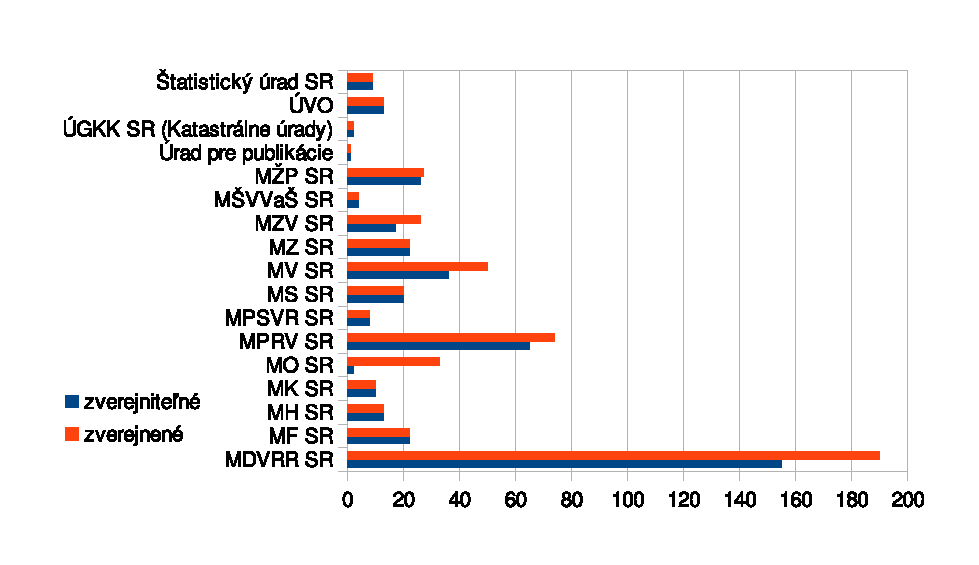
\includegraphics[width=\textwidth]{zverejnene_prevadzkovatel}
\end{frame}

\begin{frame}{Plán vs. realita (2)}{Zverejnené vs. nezverejnené}
    \begin{columns}
        \column{.5\textwidth}
        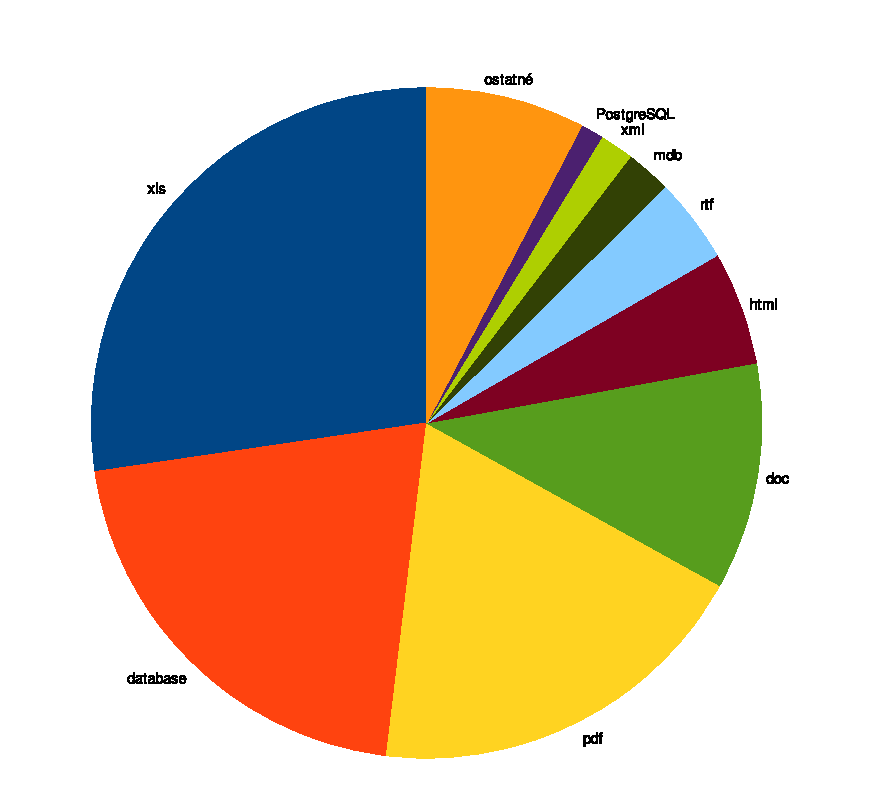
\includegraphics[width=\linewidth]{dataset_formaty}

        Formáty všetkých datasetov

        \column{.5\textwidth}
        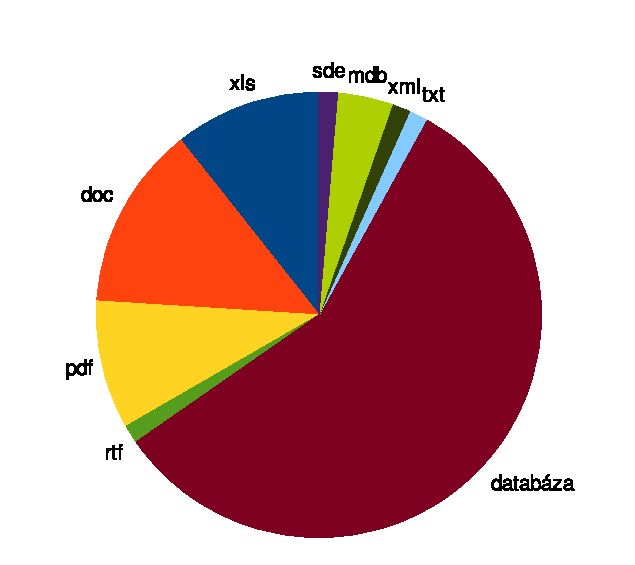
\includegraphics[width=\linewidth]{nezverejnene_formaty}

        Formáty nezverejnených datasetov
    \end{columns}
\end{frame}

\begin{frame}{Stav datasetov}
    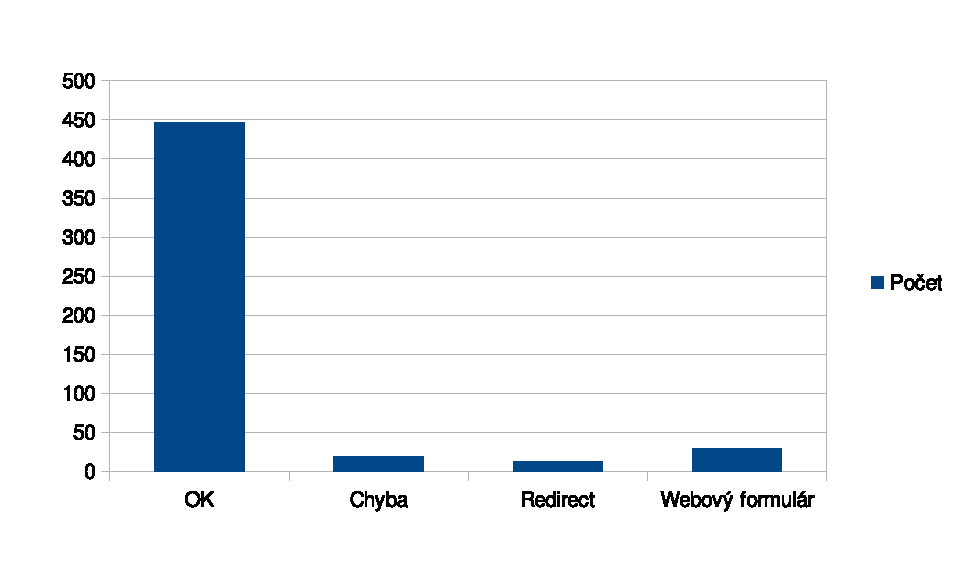
\includegraphics[width=\linewidth]{status}
\end{frame}

\begin{frame}{Hodnotenie kvality (1)}
    \begin{itemize}
        \item 5-star rating: \url{http://5stardata.info}
        \item §51, Výnos 55/2014 o~štandardoch pre informačné systémy verejnej správy
    \end{itemize}
    \begin{enumerate}
        \item dostupné na webe
        \item strojovo spracovateľné
        \item otvorený formát
        \item metadáta umožňujúce odkazovať na záznamy
        \item odkazy na záznamy v~iných datasetoch
    \end{enumerate}
\end{frame}

\begin{frame}{Hodnotenie kvality (2)}
    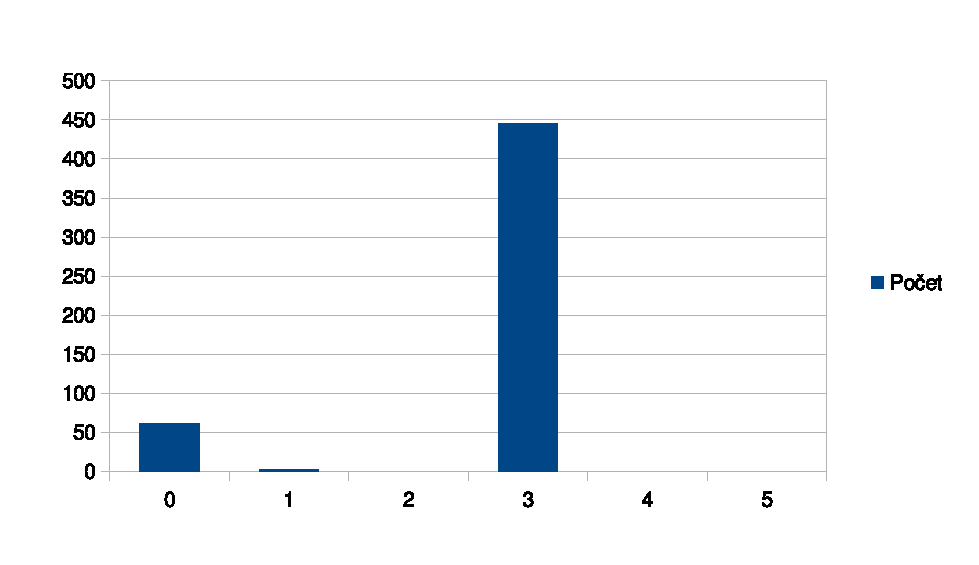
\includegraphics[width=\linewidth]{stars}
\end{frame}

\begin{frame}{Zopár pozorovaní na záver}
    \begin{itemize}
        \item technicky nič nemá ani jednu hviezdičku -- licencie
        \item CSV/XML $\not\Rightarrow$ strojová spracovateľnosť
        \item napr. zoznam datasetov: export XLS s~nekonzistentným obsahom do XML
        \item napr. zoznam faktúr MH: zle štruktúrovaná tabuľka z~Wordu, save as XML,
              pridáme RDF header
        \item podobným problémom trpí open data aj v~iných krajinách (.exe na data.gov)
        \item je potrebný systematickejší prístup: informačné systémy namiesto XLS
    \end{itemize}
\end{frame}

\end{document}
